\chapter{Méthodes itératives}
%\addcontentsline{toc}{chapter}{TD 1}


\section{Méthode de descente de gradient}

\begin{enumerate}
	\item On considère la fonction objectif $f:\RR^2 \to \RR$ suivante
	\eq{
		f(x) = \frac{1}{2}x^\top Q x \quad\text{avec}\quad Q = \begin{bmatrix} 1 & 0 \\  0& \gamma \end{bmatrix}, \quad \gamma > 0
	}
	
	\begin{enumerate}
		\item Calculer $\nabla f(x)$
		\item On cherche à minimiser $f$ par une stratégie de descente de gradient. Donner l'expression d'une itération $k$ de cet algorithme en fonction du pas $\alpha^{(k)}$.
		\item Donner l'expression de $x^{(1)}$ en fonction de $\alpha_0$ pour $x^{(0)} = [\gamma,1]^\top$.
		\item Trouver le pas optimal pour cette itération.
	\end{enumerate}
	
	\item Les figures ci-dessous montrent les résultats d'algorithmes de descente de gradient appliqués à la fonction $f$.
	\begin{enumerate}
		\item La figure~\ref{fig:descent-methods} présente l'évolution de la distance $\norm{x^{(k)}-x^{\star}}_2^2$ où $x^{\star}$ est le minimiseur global de $f$ pour trois stratégies de choix de pas: pas constant et pas optimal. Associer chaque courbe à la stratégie correspondante. Justifier votre réponse.
		
		\item La figure~\ref{fig:descent-steps} présente la valeur de la fonction $f$ au cours des itérations, dans une stratégie de pas fixe, pour différentes valeurs de pas. Commenter la figure et en déduire des recommandations pour le choix du pas de descente. Que se passe-t-il si l'on choisit un pas fixe $\alpha = 1$?
	\end{enumerate}
\end{enumerate}

\begin{figure}
\centering
		\subfloat[\label{fig:descent-methods}]{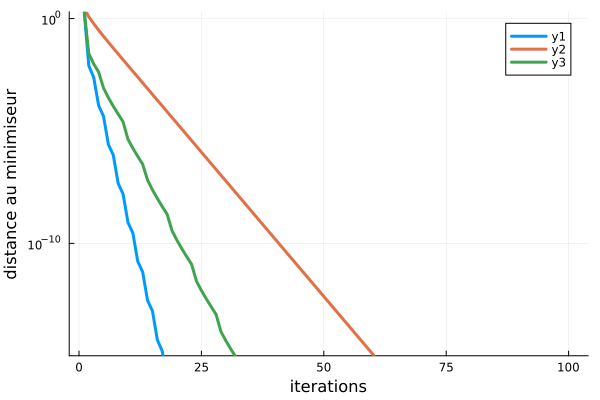
\includegraphics[width=0.47\textwidth]{td3/plots-td3-fix-opt-back-cv}} 
		\subfloat[\label{fig:descent-steps}]{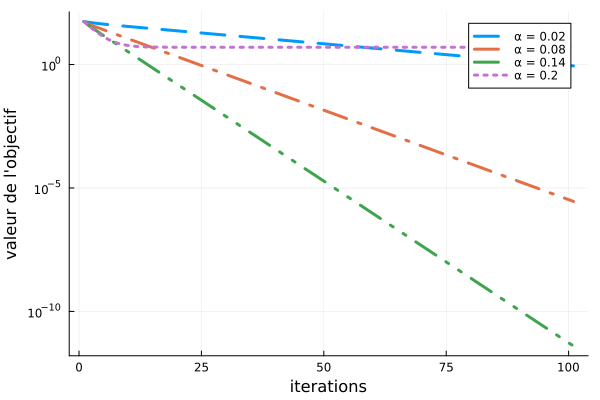
\includegraphics[width=0.47\textwidth]{td3/plots-td3-constant-cvf-initg}}
\caption{Evolution de: (a) $\norm{x^{(k)}-x^{\star}}_2^2$; (b) la fonction objectif $f$, en fonction des itérations.}
\end{figure}



\section{Méthode de Newton}

On considère la fonction $f:\RR^2 \to \RR$ définie par
\eq{
	f(x) = \frac{1}{2}x^\top Q x - b^\top x, \quad \text{avec} \quad Q \succ 0
}
\begin{enumerate}
	\item Calculer $\nabla f(x)$ et en déduire son minimiseur.
	\item Calculer $\nabla f^2(x)$.
	\item Exprimer $x^{(k+1)}$ en fonction de $x^{(k)}$ pour une itération de Newton à pas constant. Qu'en déduit-on?
\end{enumerate}
